\documentclass[12pt]{report}
\usepackage[utf8]{inputenc}
\usepackage{graphicx}
\usepackage{lipsum}
\usepackage{amsmath}
\usepackage[a4paper,left=4cm,right=2cm,top=2cm,bottom=2cm]{geometry}
\usepackage{setspace}
\usepackage{indentfirst}
\usepackage{mathptmx}
\usepackage[short]{optidef}
\usepackage{xcolor}
\usepackage{tabularx}
\usepackage{booktabs}
\usepackage[framed,numbered,autolinebreaks,useliterate]{mcode}
\graphicspath{{./graphic/}}


\onehalfspacing
\begin{document}
\begin{titlepage}
\begin{center}
\LARGE Computational Economics Problem Set I\\
\end{center}

\vskip 1in

\flushleft

By: Ruggero Jappelli and Yuna Valianta Aulia\\


\vskip 1in
\begin{center}

\end{center}
\end{titlepage}

\cleardoublepage
\pagenumbering{arabic}

\section*{Problem 1}
\subsection*{1}
\noindent
The market equilibrium is characterized by Supply = Demand. Therefore:
\begin{equation}
\begin{aligned}
& S = D\\
& a - bq = c + dq\\
& 0 = c + dq - a + bq\\
& 0 = bq + dq - (a - c)
\end{aligned}
\end{equation}

\subsection*{2}
From (1):
\begin{equation}
\begin{aligned}
& q = \frac{a - c}{b + d}
\end{aligned}
\end{equation}

Plug (2) into the demand function:
\begin{equation}
\begin{aligned}
& p = a - bq\\
& p = a - b \frac{a - c}{b + d}\\
& p = a - \frac{ab - bc}{b + d}
\end{aligned}
\end{equation}

Plug (2) into the supply function:
\begin{equation}
\begin{aligned}
& p = c + dq\\
& p = c + d \frac{a - c}{b + d}\\
& p = c + \frac{ad - cd}{b + d}
\end{aligned}
\end{equation}

\subsection*{3}
$$
\underbrace{ \begin{pmatrix}
1&b\\
1&-d\\
\end{pmatrix}}_\text{A}
\underbrace{\begin{pmatrix}
p\\
q\\
\end{pmatrix}}_\text{x}
=
\underbrace{\begin{pmatrix}
a\\
c\\
\end{pmatrix}}_\text{y}
$$

Breaking matrix A into LU:

$$
\begin{pmatrix}
1&0\\
0&1\\
\end{pmatrix}
\vline
\begin{pmatrix}
1&b\\
1&-d\\
\end{pmatrix}
\xrightarrow{r2 - r1}
\underbrace{\begin{pmatrix}
1&0\\
-1&1\\
\end{pmatrix}}_\text{L}
\vline
\underbrace{\begin{pmatrix}
1&b\\
0&-d - b\\
\end{pmatrix}}_\text{U}
$$

Therefore we can describe this as LUx = y. Let us assume Ux = z, therefore Lz = y.
$$
\underbrace{\begin{pmatrix}
1&0\\
-1&1\\
\end{pmatrix}}_\text{L}
\underbrace{\begin{pmatrix}
z_1\\
z_2\\
\end{pmatrix}}_\text{z}
=
\underbrace{\begin{pmatrix}
a\\
c\\
\end{pmatrix}}_\text{y}
$$

This will create a new system of linear equation:

\begin{equation}
\begin{aligned}
z_1 = a
\end{aligned}
\end{equation}

\begin{equation}
\begin{aligned}
-z_1 + z_2 = c \rightarrow z_2 = c - a
\end{aligned}
\end{equation}

And from Ux = z
$$
\underbrace{\begin{pmatrix}
1&b\\
0&-d - b\\
\end{pmatrix}}_\text{U}
\underbrace{\begin{pmatrix}
p\\
q\\
\end{pmatrix}}_\text{x}
=
\underbrace{\begin{pmatrix}
a\\
c - a\\
\end{pmatrix}}_\text{z}
$$

Solving for x: 
\begin{equation}
\begin{aligned}
(-d - b)q = c - a \rightarrow q = \frac{a - c}{b + d} 
\end{aligned}
\end{equation}

\begin{equation}
\begin{aligned}
p + bq = a\\
p = a - bq\\
p = a - b \frac{a - c}{b + d}
\end{aligned}
\end{equation}

\subsection*{4}
\begin{equation}
\begin{aligned}
q = \frac{a - c}{b + d} = \frac{3 - 1}{0.5 + 1}= \frac{4}{3}
\end{aligned}
\end{equation}

\begin{equation}
\begin{aligned}
p = a - b \frac{a - c}{b + d} = 3 - \frac{1}{2}\bigg(\frac{3 - 1}{0.5 + 1}\bigg) = \frac{7}{3}
\end{aligned}
\end{equation}

\subsection*{5}
Matlab code for Gauss - Seidel Method
\begin{lstlisting}
clear all
clc

%% Using Gauss - Seidel Method to solve system of lin. equation
A=[1,0.5;1,-1];
y=[3,1]';

%Choosing Q for Gauss Seidel

Q=triu(A);
Qinv = inv(Q);

tol=10e-6;
maxit=1000;
p=0.1;
q=0.1

for i=1:maxit
    p(i+1) = 3 - 0.5*q(i);
    q(i+1) = p(i+1) - 1;
    dp = p(i+1) - p(i);
    if norm(dp,1)<tol break
    end
end

disp(['The equilibrium price is ', num2str(p(end)), ' and the equilibrium quantity is ', num2str(q(end))])
disp(['The number of iteration is ', num2str(i)])
disp(' ')

\end{lstlisting}

\subsection*{6}
Matlab Code for Iteration using Succesive Over Relaxation
\begin{lstlisting}
lambda=0.1:0.1:0.9;
l=size(lambda,2);
maxit1=100000;

for j=1:l
    x1=[0,0]';
    for ii = 1:maxit1
            dx1 = Qinv*(y - A*x1);
            x1 = x1 + lambda(j)*dx1;
            if norm(dx1,1) < tol break
            end
            if ii>=maxit1
                disp('No Convergence')
            end
    end
    disp(['For lambda ', num2str(lambda(j)), ' ', ...
        ', price is ', num2str(x1(1)),', quantity is ', num2str(x1(2)),...
        ', iteration is ', num2str(ii)])
end
\end{lstlisting}

$\lambda = 0.8$ gives the fastest value of convergence.

\section*{Problem 2}
\subsection*{1 - 5}


\begin{lstlisting}
clear all
clc

%Load the quarterly GDP data from Germany and Greece
data=xlsread("OECD-Germany_Greece_GDP")';
%Log of the data
log_data = log(data);

%Separating between countries' data: Ger for German and Gre for Greece
Ger = log_data(:,1);
Gre = log_data(:,2);

%Calculating the trend from log GDP of Germany and Greece using lambda =
%1600
T_Ger = hpfilter(Ger,1600);
T_Gre = hpfilter(Gre,1600);

%Calculating the trend using OLS:
%Calculating the coefficient regressor:

%For Germany
X_Ger = [ones(length(Ger),1),(1:1:length(Ger))'];
beta_Ger = inv(X_Ger'*X_Ger)*X_Ger'*Ger;

%For Greece
X_Gre = [ones(length(Gre),1),(1:1:length(Gre))'];
beta_Gre = inv(X_Gre'*X_Gre)*X_Gre'*Gre;

%The linear trend for Germany from OLS
Y_Ger_hat = X_Ger*beta_Ger;

%The linear trend for Gre from OLS
Y_Gre_hat = X_Gre*beta_Gre;

%Calculating The Output Gap

%Germany
%Output Gap From HP Filter
Real_T_Ger = exp(T_Ger);
G_Ger_hp = (exp(Ger) - Real_T_Ger)./Real_T_Ger;
%Output Gap From OLS
Real_OLS_Ger = exp(Y_Ger_hat);
G_Ger_OLS = (exp(Ger) - Real_OLS_Ger)./Real_OLS_Ger;

%Greece
%Output Gap From HP Filter
Real_T_Gre = exp(T_Gre);
G_Gre_hp = (exp(Gre) - Real_T_Gre)./Real_T_Gre;
%Output Gap From OLS
Real_OLS_Gre = exp(Y_Gre_hat);
G_Gre_OLS = (exp(Gre) - Real_OLS_Gre)./Real_OLS_Gre;

%Plot log GDP with Hp Filter and OLS Trend
%Germany
figure('name','Log GDP versus Trends')
subplot(2,1,1)
plot(Ger)
hold on
plot(T_Ger)
plot(Y_Ger_hat,'green')
hold off
legend('Log GDP' ,'HP Filter', 'OLS','Location','southeast')
ylabel('Log GDP')
xlabel('Number of Quarters Starting from Q1 1995')
title('Log GDP, HP Filter and OLS Trend of Germany')

%Greece
subplot(2,1,2)
plot(Gre)
hold on
plot(T_Gre)
plot(Y_Gre_hat,'green')
hold off
legend('Log GDP' ,'HP Filter', 'OLS','Location','northwest')
ylabel('Log GDP')
xlabel('Number of Quarters Starting from Q1 1995')
title('Log GDP, HP Filter and OLS Trend of Greece')

%Plotting The Output Gaps from HP Filter and OLS
%Germany
figure('name','Output Gap')
subplot(2,1,1)
plot(G_Ger_hp)
hold on
plot(G_Ger_OLS)
yline(0)
hold off
legend('HP Filter' ,'OLS','Location','southeast')
ylabel('Output Gap')
xlabel('Number of Quarters Starting from Q1 1995')
title('Output Gap from HP Filter and OLS Trend of Germany')

%Greece
subplot(2,1,2)
plot(G_Gre_hp)
hold on
plot(G_Gre_OLS)
yline(0)
hold off
legend('HP Filter' ,'OLS','Location','southeast')
ylabel('Output Gap')
xlabel('Number of Quarters Starting from Q1 1995')
title('Output Gap from HP Filter and OLS Trend of Greece')

\end{lstlisting}

\subsection*{Graph for Section 2.5 (Code is at the above)}

\begin{figure}[h]
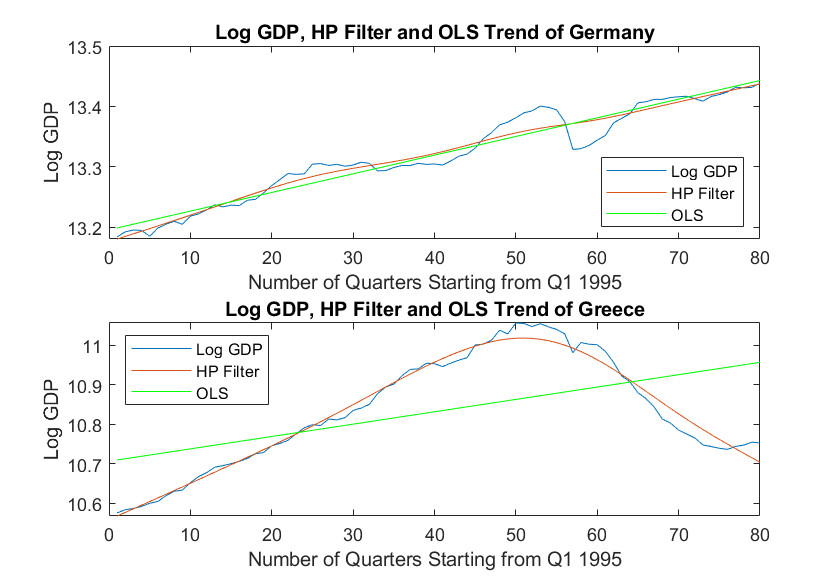
\includegraphics[height=12cm, width=\textwidth]{fig2_1}
\caption{Log GDP Versus Trend}
\end{figure}

\begin{figure}[h]
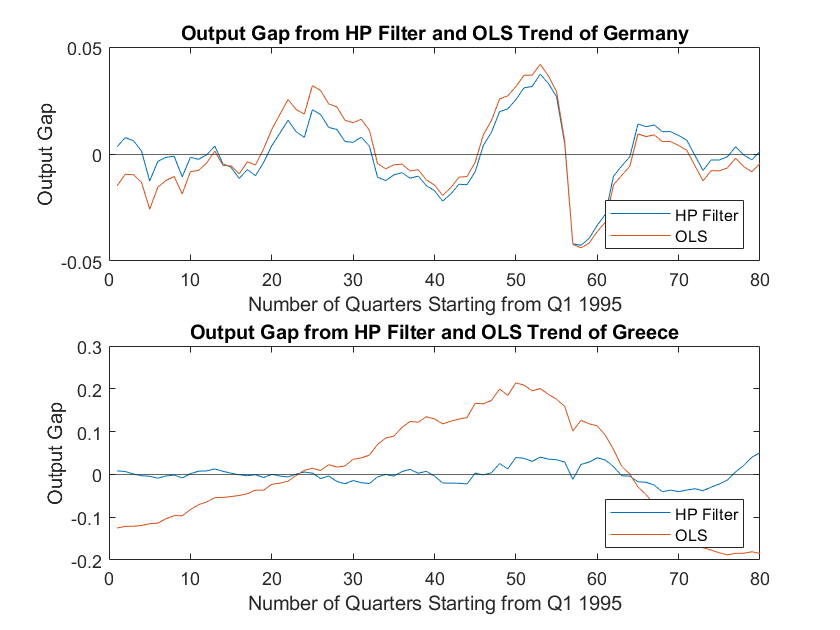
\includegraphics[height=12cm, width=\textwidth]{fig2_2}
\caption{Output Gap}
\end{figure}

\end{document}